\section{Teoria Dei Codici}
    \subsection{Introduzione}
        Ci concentriamo adesso sul trattamento dell'informazione per poterla trasmettere.
        I messaggi che trasmettiamo possono essere codificati per vari motivi:
        \begin{itemize}
            \item {
                    Compressione:$\begin{cases}
                        \text{Lossy: con perdita dell'informazione} \nonumber\\
                        \text{Lossless: minima perdita dell'informazione} \nonumber
                    \end{cases}$\\
                    Comprimere l'informazione in elimenando ridondanza e salvando spazio di memoria e banda.
                    
                }
            \item {
                    Crittografia: per nascondere il messaggio ad utenti in ascolto sul canale che non siano il destinatario.
            }
            \item {
                    Rivelazione o correzione di errore: vieen aggiunta ridondanza ad hoc per aumentare l'affidabilitá del messaggio trasmesso. 
                    Si utilizzano \href{https://en.wikipedia.org/wiki/Checksum}{checksum} o \href{https://en.wikipedia.org/wiki/Reed-Solomon_error_correction}{Reed-Solomon(RS)}
            }
        \end{itemize}
        \paragraph{Capacitá del canale}\label{Capacita del canale}\index{Capacitá del canale}
            La capacitá del canale $C$ indica la massima quantitá d'informazione che puó essere trasmessain maniera affidabile su di un dato canale.
            La capacitá dipende dalla banda $B$ del canale e dal rapporto segnale rumore (signal-to-noise ratio,\href{https://en.wikipedia.org/wiki/Signal-to-noise_ratio}{$SNR$}):
            \[
                C = B\log(1 + SNR)  
            \] 
        \paragraph{Canale Gaussiano}\index{Canale Gaussiano}
            Il canale Gaussiano puó essere modellato come \href{https://en.wikipedia.org/wiki/Binary_symmetric_channel}{Binary Symmetric Channel (BSC)} con probabilitá di errore $p$. 
            Assumiamo gli errori tra loro indipendenti ($p_{(a,b)} = p_{(a)}\dotproduct p_{(b)}$):
        \begin{figure}[H]
            \centering
            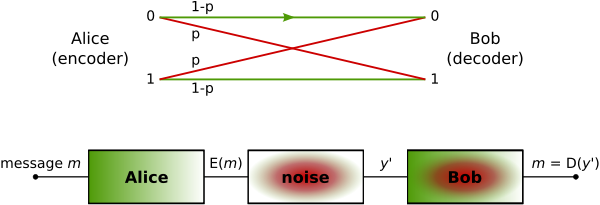
\includegraphics[width = 12cm]{media/600px-Binary_symmetric_channel_(en).svg.png}
            \label{BSC system}
            \caption{Sistema di trasmissione BSC}
        \end{figure}
        \begin{gather}
            E_{(x)}: \text{Funzione di codifica} \nonumber \\
            D_{(x)}: \text{Funzione di decodifica} \nonumber \\
            E_{(m)}: \text{Bit dell'informazione codificati} \nonumber \\
            y^\prime: E_{(m)}+ e \rightarrow \text{Informazioni con errore del canale} \nonumber \\
            m = D_{(y^\prime)}: \text{Informazione decodificata} \nonumber 
        \end{gather}
        Il canale é chiamato simmetrico perché ho la stessa probabilitá errore sulla trasmissione di uno dei due bit.
        Se $X$ é il bit inviato e Y quello ricevutoallora il canale é caratterizzato dalle probabilitá:
        \begin{align}
            P(Y=0|X=0) &= 1-p\nonumber \\
            P(Y=0|X=1) &= p\nonumber \\
            P(Y=1|X=0) &= p\nonumber \\
            P(Y=1|X=1) &= 1-p\nonumber 
        \end{align} 
        Assumiamo che $0\leq p \leq\frac{1}{2}$, se avessimo $p >\frac{1}{2}$ il ricevitore potrebbe scambiare l'informazione ricevuta
        (Quando riceve un $1$ lo interpreta come $0$ e viceversa) e ottenere un canale con probabilitá $1-p \leq\frac{1}{2}$. 
        
        Nel corso useremo delle simbologie diverse:
        \begin{figure}[H]
            \centering
            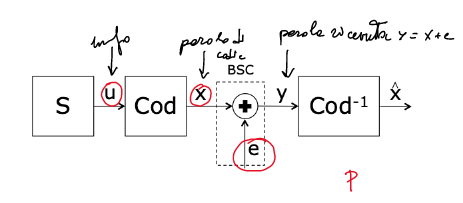
\includegraphics[width = 12cm]{media/BSC System.png}
            \label{BSC system moretti}
            \caption{Sistema di trasmissione BSC}
        \end{figure}
        \begin{gather}
            u: \text{Informazione} \nonumber \\
            x: \text{Parole di Codice} \nonumber \\
            e: \text{Errore del Canale} \nonumber \\
            y: x+e \rightarrow \text{Informazioni con errore del canale} \nonumber \\
            \overset{\wedge}{x}: \text{Informazione decodificata} \nonumber 
        \end{gather}
        \paragraph{Probabilitá di errore BSC}\label{Probabilita di errore BSC}\index{Probabilitá di errore BSC}
            La probabilitá, per una trasmissione BSC, di sbagliare $t$ bit in una parola di $n$ bit:
            \[
                p_{(t,n)} = \binom{n}{t} p^t (1-p)^{(n-t)}
            \]
            dove il coefficente binomiale:
            \[
                \binom{n}{t} = \frac{n!}{t!(n-t)!}
            \]
            indica tutte le possibili combinazioni di errori di $t$ bit su $n$ bit. 
        \paragraph{Tassonomia dei codici}
            \begin{itemize}
                \item {Codici lineari
                        \begin{itemize}
                            \item {
                                Codici a blocco
                                }
                            \item{
                                Codici convoluzionali
                            } 
                        \end{itemize}
                    }
                \item {
                    Definizione di un codice a blocco: 
                    \begin{figure}[H]
                        \centering 
                        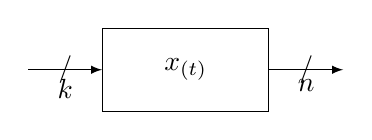
\begin{tikzpicture}[
                            node distance=2cm,
                            >=latex
                            ]

                            \node [coordinate] (input) {};
                            \node [draw, rectangle,right of = input, minimum height=3em, minimum width=6em] (block) {$x_{(t)}$};
                            \node [coordinate, right of = block] (output) {};
                            
                            \draw[draw,->] (input) -- node[midway]{$/$} node[below]{$k$} (block);
                            \draw[->] (block) -- node[midway]{$/$} node[below]{$n$} (output);
                        \end{tikzpicture}    
                    \label{Def codice a blocco}
                    \end{figure}
                    \paragraph{Rate del Codice}:\index{Rate del Codice}
                        {
                            \[
                                R = \frac{k}{n}  
                            \]
                            La condizione é che $n>k$ senon fosse cosí avrei perdita d'informazione, da $k$ bit passo a $n$ aggiungendo
                            ridondanza e codificando i miei dati. Possiamo quindi stimare il valore tipico di $R$
                            \[
                                R = \frac{k}{n} <1  
                            \]
                        }
                }
                \item Rivelazione di errore:\index{Rivelazione di errore}{
                    Consiste nella capacità di scoprire la presenza di errori causati dal rumore o da altri fenomeni deterioranti 
                    durante una trasmissione di dati (es. tramite il \href{https://it.wikipedia.org/wiki/Bit_di_parit%C3%A0}{bit di paritá}).
                }
                \item {Correzione di errore:\index{Correzione di errore}{
                    Consiste invece nell'ulteriore abilità di ricostruire i dati originali, eliminando gli errori occorsi durante la trasmissione.
                    Vi sono due differenti schemi di base per la progettazione della codifica di canale e del protocollo per un sistema che corregge gli errori:
                    \begin{itemize}
                        \item {
                            ??\href{https://it.wikipedia.org/wiki/Automatic_repeat-request}{Automatic repeat-request} (ARQ): Il mittente invia i dati ed anche un codice a rilevazione d'errore, che sarà
                            utilizzato in ricezione per individuare gli eventuali errori, ed in tal caso chiedere la ritrasmissione dei dati
                            corrotti. In molti casi la richiesta è implicita; il destinatario invia un acknowledgement (ACK) di corretta 
                            ricezione dei dati, ed il mittente re-invia solo quei dati per i quali non ha ricevuto, entro un prefissato tempo 
                            limite (timeout), il corrispondente ACK.
                        }
                        \item{
                            ??\href{https://it.wikipedia.org/wiki/Forward_Error_Correction}{Forward Error Correction} (FEC): Il mittente codifica i dati con un codice a correzione d'errore 
                            (error correction code, ECC) ed invia il messaggio codificato. Il destinatario non invia mai alcun 
                            messaggio verso il mittente; esso decodifica ciò che riceve nella maniera più simile possibile a quella di un 
                            certo insieme prefissato di parole accettabili. Tali codici sono realizzati in modo tale che dovrebbe occorrere 
                            una quantità "irragionevole" di errori nei dati, affinché il destinatario decodifichi erroneamente, ottenendo 
                            finalmente dei dati diversi da quelli effettivamente inviatigli.
                        } 
                    \end{itemize}
                    In generale un codice a blocco che ha rate $\frac{k}{n}$ mappa $k$ bit su $n$ bit usando $2^k$ parole di codice di dimensione n
                }}
            \end{itemize}

        \subsubsection{Esempio codici a blocco: codici a ripetizione}
            É un esempio di codice a correzione d'errore: il funzionamento si basa sulal ripetizione dell'informazione piú volte. Il destinatario
            si accorge di un errore di trasmissione poiché il flusso di dati ricevuto non è la ripetizione di un singolo messaggio e, inoltre, 
            il destinatario può recuperare il messaggio originale guardando il messaggio ricevuto nel flusso di dati che si verifica più spesso.

            Nel caso di un codice binario di ripetizione, esistono due parole in codice - tutte uno e tutti zeri - che hanno una lunghezza n. 
            Pertanto, la distanza minima di Hamming (\ref{Distanza di Hamming}) del codice è uguale alla sua lunghezza. Ciò conferisce al codice 
            di ripetizione, con $R = \frac{1}{n}$,una capacità di rivelazione di errori pari a $n-1$ e correzione degli errori (cioè correggerà fino agli errori in qualsiasi parola del codice) di $\frac{n-1}{2}$ per n dispari(\ref{Probabilita di errore BSC}).\\
            Esempio:\\
            \indent{$R = \frac{1}{3} \rightarrow$ ha solo 2 parole di codice:}
            \begin{align}
                u=0 \rightarrow x = [000]\nonumber \\
                u=1 \rightarrow x = [111]\nonumber
            \end{align} 
            Il ricevitore effettua una decodifica a maggioranza: decideper il bitche comprare nella maggioranzadalle posizionidella parola ricevuta.
            \begin{align}
                y = [000] \rightarrow \overset{\wedge}{x} = [000] \rightarrow \overset{\wedge}{u} = 0 \nonumber \\
                y = [010] \rightarrow \overset{\wedge}{x} = [000] \rightarrow \overset{\wedge}{u} = 0 \nonumber \\
                y = [101] \rightarrow \overset{\wedge}{x} = [111] \rightarrow \overset{\wedge}{u} = 1 \nonumber
            \end{align}

        \subsubsection{Esempio codici a blocco: codici a controllo di paritá}

        \subsubsection{Esempio codici a blocco: codice ISBN}
    \subsection{Codici a blocco}
        \subsubsection{Introduzione ai codici lineari}
            {Definizione di campo}
        \subsubsection{Campi di Galois}

        \subsubsection{Codici a blocco lineari su $GF(2)$}
        n>k perché nei codici io metto cose in piú che magari non mi servono amplio le cose.\\


        \subsubsection{Propietá dei codici a blocco lineari}
            \begin{itemize}
                \item {1}
                \item {2}
                \item {3}
                \item {4}
                \item {5}
            \end{itemize}
        \subsubsection{Distanza di Hamming}\label{Distanza di Hamming}\index{Distanza di Hamming}
            

            Peso di hamming.
            distanza minima di un codice

        \subsubsection{Codici a blocco in forma sistematica}
            \begin{itemize}
                \item {1 matrici che generano codici equivalenti }
                \item {2 qualsiasi codice lineare a blocchi é equivalente a un codice in forma sistematica}
                \item {3}
                \item {4}
                \item {5}
                \item {6 codici equivalenti}
            \end{itemize}

        se non é una parola di codice la matrice H ci informa con un vaolre 1 nel prodottod